\scanpage{43}
\mspage{\handwritten{11}}
\uline{11.- Préschémas en groupes affines.}

\uline{\handwritten{11}.0.}- Notations : soient $S$ un préschéma, $X$ un $S$-préschéma, $f:X\handwritten{\to}S$ le morphisme structural; on pose $\handwritten{\unsure{\mathcal{A}|a}}(X)=f_{\handwritten{*}}(\handwritten{\mathcal{O}}_X)$.

\handwritten{\makebox[0pt][l]{\raisebox{-2ex}{\begin{tikzpicture}[x=1cm,y=1cm]\draw (.05,.14) -- (.05,-.07) -- (.13,-.07);\end{tikzpicture}}}}\uline{Lemme 11.1.- Soient $X$ et $Y$ deux $S$-préschémas quasi-compacts et quasi-séparés sur $S$, $f:X\handwritten{\to}S$ et $g:Y\handwritten{\to}S$ les morphismes structuraux. Alors l'homomorphisme canonique}
\[
\handwritten{\varphi}:\handwritten{\mathcal{A}}(X)\handwritten{\otimes}_{\handwritten{\mathcal{O}}_{\unsure{\mathbb{S}|S}}}\handwritten{\mathcal{A}}(Y)\handwritten{\longrightarrow}\handwritten{\mathcal{A}}(X\handwritten{\times}_S Y)
\]
% Curved pen mark below the tensor-base index.
\figure{\handwritten{\begin{tikzpicture}[x=1cm,y=1cm]\draw (0,.18) .. controls (.25,-.2) and (.8,-.18) .. (1.25,.22);\end{tikzpicture}}}
\margin{\handwritten{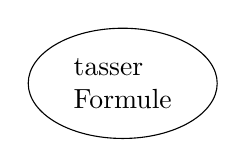
\begin{tikzpicture}[x=1cm,y=1cm]
\draw (0,0) ellipse (1.2 and .7);
\node[align=left] at (0,0) {tasser\\Formule};
\end{tikzpicture}}}
\uline{est un isomorphisme dans chacun des cas suivants :}

\uline{a) $f$ et $g$ sont affines}

\uline{b) $f$ ou $g$ est plat et affine}

\uline{c) $g$ est plat et $f_{\handwritten{*}}(\handwritten{\mathcal{O}}_X)$ est un $\handwritten{\mathcal{O}}_S$-Module plat.}
% Curved pen mark below the star of f in c).
\figure{\handwritten{\begin{tikzpicture}[x=1cm,y=1cm]\draw (0,.15) .. controls (.15,-.16) and (.45,-.16) .. (.6,.16);\end{tikzpicture}}}
\margin{\handwritten{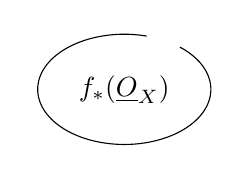
\begin{tikzpicture}[x=1cm,y=1cm]
\draw (.285,.676) arc[start angle=75,end angle=410,x radius=1.1,y radius=.7];
\node at (0,0) {$f_*(\underline{O}_X)$};
\end{tikzpicture}}}

Dans le cas b), on peut supposer que c'est $g$ qui est plat et affine. Posons $S'=\operatorname{Spec}\handwritten{\mathcal{A}}(X)$ $Y'=Y\handwritten{\times}_S\unsure{\mathbb{S}|S}'$, $g'=g\handwritten{\times}_S S'$ et notons $v$ le morphisme $S'\handwritten{\to}S$. Alors $Y$ est quasi-compact et quasi-\linebreak -séparé sur $S$, et, ou bien $S'$est plat sur $S$ (cas c) d'après (EGA III (1.4.15.5)), ou bien $g$ est affine (cas a) et b)). Alors (EGA III 1.4.15 et IV 1.2.7 ou II 1.5.2), on a :
\[
g'_{\handwritten{*}}(\handwritten{\mathcal{O}}_{Y'})=v^{\handwritten{*}}g_{\handwritten{*}}(\handwritten{\mathcal{O}}_Y)=\handwritten{\mathcal{A}}(Y)\handwritten{\otimes}_{\handwritten{\mathcal{O}}_S}\handwritten{\mathcal{O}}_{S'}.
\]

D'après (EGA II 1.2.7), $f$ se \unsure{factorise|favtorise} à travers $v$ au moyen \handwritten{\makebox[0pt][l]{\raisebox{2ex}{\begin{tikzpicture}[x=1cm,y=1cm]\draw (0,0) -- (.17,.09) -- (.43,-.05);\end{tikzpicture}}}}d'un morphisme $p:G\handwritten{\to}S'$, et on a : $X\handwritten{\times}_S Y=X\handwritten{\times}_{S'}Y'$ et $p_{\handwritten{*}}(\handwritten{\mathcal{O}}_X)=\handwritten{\mathcal{O}}_{S'}$. Puisque $v$ et $f$ sont quasi-compacts et quasi-séparés,\deleted{sur} il en est de même de $p$ (EGA IV 1.2.2 et 1.2.4)\handwritten{;} \handwritten{O}u bien $Y$ est plat sur $S$ (cas b) et c)) et alors $Y'$ est plat sur $S'$, ou bien $X$ est affine sur $S$ (cas a)), et alors $p$ est un isomorphisme. Dans le premier cas, on peut de nouveau appliquer (EGA III 1.4.15 et IV 1.2.7), et dans les deux cas, on trouve :
\[
\deleted{\unsure{p_*|q_*}\ \unsure{=}\ \unsure{q'_*|p'_*}}\ p'_{\handwritten{*}}(\handwritten{\mathcal{O}}_{X\handwritten{\times}_S Y})=g'^{\handwritten{*}}p_{\handwritten{*}}(\handwritten{\mathcal{O}}_X)=g'^{\handwritten{*}}(\handwritten{\mathcal{O}}_{S'})=\handwritten{\mathcal{O}}_{Y'}\handwritten{,\ \text{ou }p'=p\times_{S'}Y'.}
\]

D'où :
\[
\handwritten{\mathcal{A}}(X\handwritten{\times}_S Y)=v_{\handwritten{*}}g'_{\handwritten{*}}p'_{\handwritten{*}}(\handwritten{\mathcal{O}}_{X\handwritten{\times}_S Y})=v_{\handwritten{*}}g'_{\handwritten{*}}(\handwritten{\mathcal{O}}_{\handwritten{Y}'})=v_{\handwritten{*}}(\handwritten{\mathcal{A}}(Y)\handwritten{\otimes}_{\handwritten{\mathcal{O}}_S}\handwritten{\mathcal{O}}_{S'})=\handwritten{\mathcal{A}}(Y)\handwritten{\otimes}_{\handwritten{\mathcal{O}}_S}\handwritten{\mathcal{A}}(X)
\]
d'après (EGA II 1.4.7).

\uline{Corollaire 11\handwritten{\unsure{.|/}}2.- On définit un foncteur $X\handwritten{\rightsquigarrow}\operatorname{Spec}\handwritten{\mathcal{A}}(X)$ de la sous-catégorie pleine de $\operatorname{Sch}_{/S}$ des $X$-préschémas plats quasi-compacts et quasi-séparés sur $S$ tels que $\handwritten{\mathcal{A}}(X)$ soit un $\handwritten{\mathcal{O}}_S$-Module plat , dans celle des $S$-préschémas plats et affines sur $S$ . Ce foncteur commute aux produits finis, donc transforme $S$-groupes en $S$-groupes.}
% archive sheet number: 42
